\chapter{Phần cứng và phần mềm}

Lập trình nhúng rất gần với phần cứng, nên để hiểu rõ được chương trình nhúng cần hiểu rõ phần cứng, cấu trúc bên trong của vi xử lí, cách một CPU chạy, cách quản lí tài nguyên\dots

Chương này mình sẽ giới thiệu sơ lược về bộ nhớ, con trỏ và các khía cạnh khác của ngôn ngữ C. Ngôn ngữ C ra đời từ rất lâu, khi máy tính có cấu hình rất hạn chế, việc lập trình đòi hỏi phải tiết kiệm đến từ bit, byte bộ nhớ. Khi các máy tính mạnh dần, việc can thiệp sâu vào phần cứng để tối ưu hóa trở nên thừa thãi và phức tạp đến mức không cần thiết. Các ngôn ngữ hiện đại sau này như python, java, C\# đều không tiếp xúc quá sâu vào phần cứng như C mà tập trung vào xây dựng các thư viện tiện dụng.

Thế nên các công cụ đặc trưng của C hiện tại chỉ thích hợp cho các chip với cấu hình nhỏ, giá rẻ trong các vi mạch nhúng, hoặc các thuật toán đòi hỏi độ tối ưu hóa cao trên máy tính.

\section{Cơ bản về chương trình}
 
Việc lập trình là chỉ cho cái máy biết bạn muốn nó làm gì.

Khi bạn viết chương trình, bên dịch thì máy tính sẽ biên dịch code của bạn (người hiểu được) thành mã máy (máy hiểu được) bao gồm các lệnh mà vi điều khiển sẽ thực và khi nạp xuống cho vi điều khiển thì chương trình sẽ được lưu ở bộ nhớ chương trình. CPU sẽ đọc lệnh từ bộ nhớ chương trình rồi thực thi. Lưu ý là CPU chỉ đọc thôi, nó không được phép ghi gì vào bộ nhớ chương trình. Thế nên bộ nhớ chương trình có tên là bộ nhớ chỉ đọc (Read-only memory, ROM). Bộ nhớ chương trình không bị mất đi khi mất điện.

Còn bộ nhớ RAM là bộ nhớ phục vụ cho chương trình khi chương trình đang chạy.

Ví dụ như bạn khai báo biến int a=0; thì biến a sẽ được lưu trong RAM. Sau đó có lệnh a=a+1; CPU sẽ lấy biến a từ trong RAM ra, thực hiện phép tính rồi lại lưu vào chỗ cũ.

Do việc RAM được CPU sử dụng để thực hiện chương trình, đọc ghi liên tục nên nó gọi là bộ nhớ truy cập ngẫu nhiên (Random-access Memory) CPU đươc toàn quyền sử dụng bộ nhớ này. Khi mất điện thì chương trình phải chạy lại từ đầu nên những gì được lưu trong làm là không cần thiết và bị xóa trắng. Có một số chip có một vùng RAM nhỏ được nuôi bằng pin để lưu một vài thông số quan trọng, khi có điện lại thì chương trình đọc các thông số đó ra và chạy tiếp. Ví dụ như một dây chuyền sản xuất, nó phải lưu lại vị trí của dây chuyền để khi có điện có thể chạy tiếp.

\section{Về cách tổ chức bộ nhớ}

Thông thường thì đơn vị nhỏ nhất của bộ nhớ là byte (mà mình hay gọi là ô nhớ), mỗi byte được đánh một địa chỉ. Tùy số lượng bit của bus địa chỉ mà quyết định xem nó có thể quản lý bao nhiêu ô nhớ. Nếu bus địa chỉ 8-bit thì nó có thể quản lý 256 byte bộ nhớ, bus địa chỉ 16-bit thì có thể quản lý 64kbyte, còn 32-bit thì có thể quản lý tới 4Gbyte bộ nhớ. 

\begin{figure}[h!]
\centering

%\label{fig:Bộ nhớ 16 bit}
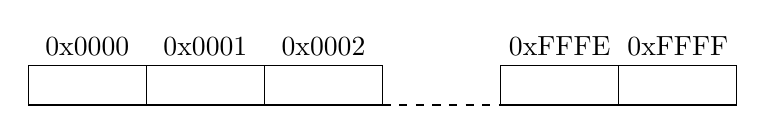
\begin{tikzpicture}[yscale=0.5, xscale=1.5]

    \draw (0,0) rectangle (1,1);
    \draw (1,0) rectangle (2,1);
    \draw (2,0) rectangle (3,1);
    \draw [dashed] (3,0) -- (4,0);
    \draw (4,0) rectangle (5,1);
    \draw (5,0) rectangle (6,1);
    \node  [above] at (0.5, 1) {0x0000};
    \node  [above] at (1.5, 1) {0x0001};
    \node  [above] at (2.5, 1) {0x0002};
    \node  [above] at (4.5, 1) {0xFFFE};
    \node  [above] at (5.5, 1) {0xFFFF};
\end{tikzpicture}
\caption{Bộ nhớ địa chỉ 16-bit} 
\end{figure}

Vậy mỗi ô nhớ sẽ có 2 thông số mà bạn cần quan tâm: 
\begin{itemize}
    \item Địa chỉ: nó ở đâu, địa chỉ có thể là số 8-bit, 16-bit, 32-bit... và số này là không đổi.
    \item Và giá trị được lưu: nó bao nhiêu, chỉ là số 8-bit (1 byte). Mỗi khi bạn lưu một số mới thì giá trị được lưu sẽ thay đổi.
\end{itemize}

\begin{figure}[h!]
\centering
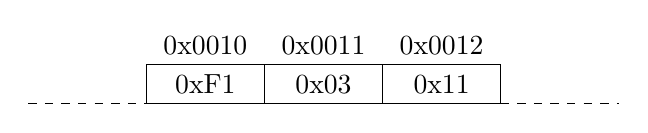
\begin{tikzpicture}[yscale=0.5, xscale=1.5]
    \draw [dashed] (0,0) -- (1,0);
    \draw (1,0) rectangle (2,1);
    \draw (2,0) rectangle (3,1);
    \draw (3,0) rectangle (4,1);
    \draw [dashed] (4,0) -- (5,0);
    
    \node  [above] at (1.5, 1) {0x0010};
    \node  [above] at (2.5, 1) {0x0011};
    \node  [above] at (3.5, 1) {0x0012};
    \node   at (1.5, 0.5) {0xF1};
    \node   at (2.5, 0.5) {0x03};
    \node   at (3.5, 0.5) {0x11};

\end{tikzpicture}
\caption{Dữ liệu trong bộ nhớ} %\label{fig: Dữ liệu trong bộ nhớ}
\end{figure}

Đoạn chương trình để xem địa chỉ trong DevC++:\*
\begin{lstlisting}
#include <stdio.h>
void main(){
    char a;
    printf("a address: 0x%08x\n", &a);
}
\end{lstlisting}


\section{Khai báo biến}

Các kiểu biến thông thường khi lập trình C là char, int, long, float, double. Nhưng trong lập trình nhúng, tài nguyên bộ nhớ hạn chế nên việc bạn biết các biến chiếm bao nhiêu ô nhớ là điều rất quan trọng. Thông thường, các biến được khai báo dưới dạng \it{uint8\_t}, \it{int8\_t}, \it{uint16\_t}, \it{int16\_t}... để sử dụng thì bạn cần thêm vào thư viện \it{\#include <stdint.h>}

Một điểm đặc biệt là kiểu \it{uint8\_t} thường được dùng để đại diện cho một ô nhớ (8-bit). Ví dụ khi khai báo \it{uint8\_t array[3]}, thì có thể hiểu là khai báo 3 phần tử mảng array có kiểu là \it{uint8\_t}, hoặc cũng có thể hiểu là yêu cầu bộ nhớ cấp 3 ô nhớ kề nhau. Các kiểu như byte hoặc char cũng có thể được dùng làm việc này nhưng mình vẫn thích sử dụng \it{uint8\_t}. Các khai báo các bộ đệm trong các giao tiếp như uart, i2c, spi... thường dùng kiểu biến này.

Thế nên hãy thường sử dụng các kiểu dữ liệu với bộ nhớ tường minh trên để kiểm soát bộ nhớ chặt chẽ hơn.

\section{Kiểu dữ liệu tự định nghĩa}

Ngôn ngữ C cung cấp cơ chế tự định nghĩa kiểu dữ liệu để việc truy xuất dữ liệu được thuận tiện.

Ví dụ mình có một cái cảm biến có thể đọc về nhiệt độ, độ ẩm và ánh sáng môi trường. Dữ liệu nhiệt độ từ  -20\textdegree{}C đến 100\textdegree{}C, độ ẩm từ 0\% đến 100\%, ánh sáng từ 0 lux đến 50.000 lux. Vậy mình khai báo dữ kiểu dữ liệu env\_t (viết tắt của environment) như sau:

\begin{lstlisting}
typedef struct{
    int8_t temp;
    uint8_t humi;
    uint16_t lux;
}env_t;
\end{lstlisting}

Dễ thấy là các kiểu biến bên trong đều chứa đủ khoảng giá trị cần thiết (nếu nhiệt độ vượt quá 127\textdegree{}C thì biến int8\_t không chứa được, phải chọn kiểu khác).

Thực chất kiểu dữ liệu là cách bạn tương tác với một vùng nhớ cho trước. Ví dụ khi khai báo một biến như \textit{env\_t env;} chẳng hạn, nó sẽ cung cấp cho bạn 4 ô nhớ liền nhau. Nếu bạn in địa chỉ của biến env ra nó sẽ hiển thị địa chỉ ô nhớ \textit{đầu tiên} của dãy 4 ô nhớ đó. Và kiểu env\_t sẽ cho máy tính biết cách truy cập tới 4 ô nhớ đó như thế nào.

\begin{figure}[h!]
\centering
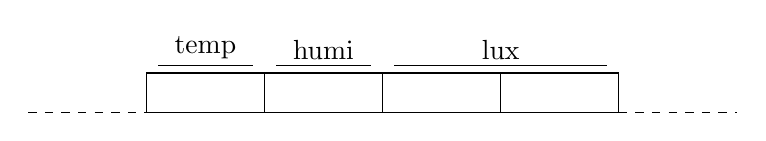
\begin{tikzpicture}[yscale=0.5, xscale=1.5]
    \draw [dashed] (0,0) -- (1,0);
    \draw (1,0) rectangle (2,1);
    \draw (2,0) rectangle (3,1);
    \draw (3,0) rectangle (4,1);
    \draw (4,0) rectangle (5,1);
    \draw [dashed] (5,0) -- (6,0);
    
    \draw (1.1, 1.2) -- (1.9, 1.2);
    \node [above] at (1.5, 1.1) {temp};
    
    \draw (2.1, 1.2) -- (2.9, 1.2);
    \node [above] at (2.5, 1.1) {humi};
    
    \draw (3.1, 1.2) -- (4.9, 1.2);
    \node [above] at (4, 1.1) {lux};
    
\end{tikzpicture}
\caption{Truy cập biến kiểu env\_t} %\label{fig: Dữ liệu trong bộ nhớ}
\end{figure}

Đoạn chương trình xem độ dài của kiểu dữ liệu:

\begin{lstlisting}
#include <stdio.h>
#include <stdint.h>

typedef struct{
    int8_t temp;
    uint8_t humi;
    uint16_t lux;
}env_t;

void main(void) {
printf("Size of env_t: %d\n", sizeof(env_t));
}
\end{lstlisting}

Một điểm cần lưu ý là các máy tính thường có cơ chế làm tròn biên kiểu dữ liệu (data structure alignment). Nếu chúng ta khai báo như sau:

\begin{lstlisting}
typedef struct{
    int8_t temp;
    uint16_t lux;
    uint8_t humi;
}env_t;
\end{lstlisting}

biến lux khai báo ở giữa, thì kiểu dữ liệu env\_t giờ đây có độ dài là 6 byte chứ không phải 4!!!.

Kiểu biến env\_t giờ có cấu trúc như sau:

\begin{figure}[h!]
\centering
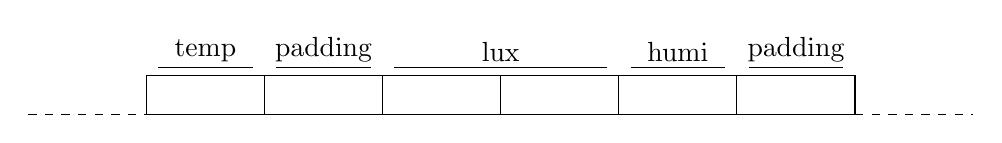
\begin{tikzpicture}[yscale=0.5, xscale=1.5]
    \draw [dashed] (0,0) -- (1,0);
    \draw (1,0) rectangle (2,1);
    \draw (2,0) rectangle (3,1);
    \draw (3,0) rectangle (4,1);
    \draw (4,0) rectangle (5,1);
    \draw (5,0) rectangle (6,1);
    \draw (6,0) rectangle (7,1);
    \draw [dashed] (7,0) -- (8,0);
    
    \draw (1.1, 1.2) -- (1.9, 1.2);
    \node [above] at (1.5, 1.1) {temp};
    
    \draw (2.1, 1.2) -- (2.9, 1.2);
    \node [above] at (2.5, 1.1) {padding};
    
    \draw (3.1, 1.2) -- (4.9, 1.2);
    \node [above] at (4, 1.1) {lux};
    
    \draw (5.1, 1.2) -- (5.9, 1.2);
    \node [above] at (5.5, 1.1) {humi};
    
    \draw (6.1, 1.2) -- (6.9, 1.2);
    \node [above] at (6.5, 1.1) {padding};
\end{tikzpicture}
\caption{Truy cập biến kiểu env\_t} 
\end{figure}

Hai ô nhớ tên \textit{padding} được thêm vào để tăng hiệu suất việc đọc ghi dữ liệu trong máy tính hiện đại. Các bạn quan tâm thì có thể tìm hiểu thêm. 

Ta thể tránh nó bằng cách khai báo như sau: trong DevC++ thì bạn khai báo \textit{\#pragma pack(1)} trước khi khai báo biến dữ liệu, còn trong nếu sử dụng KeilC cho chip STM32 thì khai báo kiểu:

\begin{lstlisting}
typedef __packed struct{
    int8_t temp;
    uint16_t lux;
    uint8_t humi;
}env_t;
\end{lstlisting}

mỗi khi khai báo một kiểu biến nào đó. Việc này áp dụng cho những dòng chip 16 bit, 32 bit, 64 bit. Còn Arduino là chip 8 bit nên không có cơ chế này.

\section{Con trỏ}

Có thể nói con trỏ là công cụ lợi hại nhất của C, bạn khó mà giỏi C nếu bỏ qua con trỏ được. Bản chất của con trỏ (chưa nói đến con trỏ hàm) là trỏ tới một vùng nhớ nào đó và tương tác với vùng nhớ đó. Chương trình ví dụ về con trỏ:

\begin{lstlisting}
#include <stdio.h>
#include <stdint.h>

int main(void) {
    uint16_t a=0;
    uint16_t *pa;
    pa=&a;
    printf("a addr: 0x%08x\n", &a);
    printf("a addr: 0x%08x\n", pa);
}
\end{lstlisting}

Hai lần printf sẽ cho ra kết quả như nhau vì đã gán địa chỉ của a cho pa.

Một con trỏ cần 2 thông tin sau để có thể hoạt động được: \textit{địa chỉ} và \textit{kiểu dữ liệu} nó sẽ trỏ tới. Như chương trình trên thì dòng số 6 sẽ cấp cho con trỏ kiểu dữ liệu, dòng số 7 cấp địa chỉ. 2 yếu tố trên giúp bạn có thể đi đến vùng nhớ mà bạn quan tâm sau đó có thể truy cập vùng nhớ đó theo cách bạn muốn.

\section{Ví dụ về truyền nhận UART}

Để biết con trỏ nó lợi hại như thế nào thì các bạn hãy xem ví dụ về truyền nhận UART. Các hàm truyền nhận dữ liệu UART thường có cấu trúc như sau:

\begin{lstlisting}
uart_transmit(uint8_t *data, uint16_t size);
uart_receive(uint8_t *data, uint16_t size);
\end{lstlisting}

Trong hàm uart\_transmit, tham số *data là ô nhớ đầu tiên trong chuỗi ô nhớ liên tiếp mà bạn muốn gửi đi. Còn trong hàm uart\_receive, tham số *data là ô nhớ đầu tiên của vùng nhớ mà bạn sẽ cất dữ liệu nhận được vào đấy (địa chỉ bộ đệm).

Mình ví dụ chương trình sau: một MCU đọc các dữ liệu cảm biến môi trường rồi truyền qua đường UART về một MCU khác để xử lý. Đây là bài toán điển hình cho một mạng gồm nhiều node cảm biến khác nhau và gửi về bộ xử lí trung tâm.

Các bước thực hiện của mình như sau:
\begin{itemize}
    \item Khai bao một biến kiểu \textit{env\_t} rồi gắn dữ liệu cho biến này.
    \item Do UART mỗi lần chỉ gửi được 1 byte, mà dữ liệu ta cần tới 4 byte, ta phải rã dữ liệu của ta ra thành từng byte một và gửi đi.
    \item Bên nhận cũng nhận từng byte một và  sau đó ghép lại thành dữ liệu hoàn chỉnh.
\end{itemize}

Chương trình khai báo và gắn dữ liệu vào biến:
\begin{lstlisting}
env_t env;
env.temp=20;
env.humi=80;
env.lux=10000;
\end{lstlisting}

Sau khi có dữ liệu, để chuyển đi ta cần rã dữ liệu ra thành từng byte một bằng cách khai báo một con trỏ kiểu \it{uint8\_t} và trỏ đến địa chỉ của biến \it{env}.

\begin{lstlisting}
uint8_t *p_env=(uint8_t *)&env;
\end{lstlisting}

Thật ra chúng ta chỉ thay đổi \it{cách chúng ta đọc bộ nhớ}, không thay đổi giá được lưu trong ô nhớ RAM. Như hình 1.5 là cách 2 kiểu biến nhìn các ô nhớ trong RAM.

\begin{figure}[h!]
    \centering
    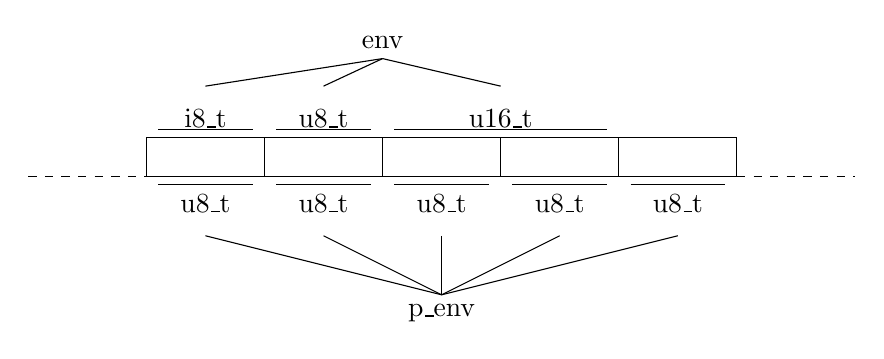
\begin{tikzpicture}[yscale=0.5, xscale=1.5]
        \draw [dashed] (0,0) -- (1,0);
        \draw (1,0) rectangle (2,1);
        \draw (2,0) rectangle (3,1);
        \draw (3,0) rectangle (4,1);
        \draw (4,0) rectangle (5,1);
        \draw (5,0) rectangle (6,1);
        \draw [dashed] (6,0) -- (7,0);
        
        \draw (1.1, 1.2) -- (1.9, 1.2);
        \node [above] at (1.5, 1) {i8\_t};
        \draw (1.5,2.3)--(3,3);		
        
        \draw (2.1, 1.2) -- (2.9, 1.2);
        \node [above] at (2.5, 1) {u8\_t};
        \draw (2.5,2.3)--(3,3);		
        
        \draw (3.1, 1.2) -- (4.9, 1.2);
        \node [above] at (4, 1) {u16\_t};
        \draw (4,2.3)--(3,3);	
        
        \node [above] at (3, 3) {env};
        
        \draw (1.1, -0.2) --(1.9,-0.2);
        \node [below] at (1.5, -0.2) {u8\_t};
        \draw (1.5, -1.5) -- (3.5,-3);
    
        \draw (2.1, -0.2) --(2.9,-0.2);
        \node [below] at (2.5, -0.2) {u8\_t};
        \draw (2.5, -1.5) -- (3.5,-3);
    
        \draw (3.1, -0.2) --(3.9,-0.2);
        \node [below] at (3.5, -0.2) {u8\_t};
        \draw (3.5, -1.5) -- (3.5,-3);
    
        \draw (4.1, -0.2) --(4.9,-0.2);
        \node [below] at (4.5, -0.2) {u8\_t};
        \draw (4.5, -1.5) -- (3.5,-3);
    
        \draw (5.1, -0.2) --(5.9,-0.2);
        \node [below] at (5.5, -0.2) {u8\_t};
        \draw (5.5, -1.5) -- (3.5,-3);
        
        \node [below] at (3.5, -3) {p\_env};
        
    \end{tikzpicture}
\caption{Buffer v.s env\_t.}
\end{figure}

Như ta thấy cùng một giá trị của ô nhớ RAM nhưng cách ta đọc khác nhau thì cho về kết quả khác nhau.

Do giới hạn trọng việc demo nên mình sẽ mô phỏng truyền nhận dữ liệu như sau:

\begin{lstlisting}
uint8_t rx_buffer[10];
for(uint8_t i=0; i<sizeof(env_t); i++){
    rx_buffer[i]=*(p_env+i);
}
\end{lstlisting}

Vòng lặp \it{for} sẽ copy theo thứ tự tất cả các byte của biến \it{env} vào bộ đêm \it{rx\_buffer}. Và công việc cuối cùng là đọc lại dữ liệu ban đầu từ bộ đệm \it{rx\_buffer}.

\begin{lstlisting}
env_t *rx_env=(env_t *)rx_buffer;
debug("Received temperature: %d\n",rx_env->temp);
debug("Received humidity: %d\n",rx_env->humi);
debug("Received lux: %d\n",rx_env->lux);
\end{lstlisting}

Việc đọc lại bằng cách ngược lại, khai báo con trỏ kiểu \it{env\_t} rồi trỏ vào bộ đệm \it{rx\_buffer}.

Ở trên mình vừa trình bày con trỏ, kiểu dữ liệu tự định nghĩa. Đây là hai công cụ giúp bạn có thể tiếp xúc rất sâu vào bộ nhớ máy tính và là một trong những đặc trưng của ngôn ngữ C.

